\documentclass{beamer}
\usetheme{Boadilla}

\usepackage{graphicx}
\usepackage{subcaption}
\usepackage{csvsimple}
 The R package coloc performs colocalization tests between genetic traits:
https://CRAN.R-project.org/package=coloc
% Change size of footnotes
\renewcommand{\footnotesize}{\fontsize{5pt}{5pt}\selectfont}
\title{Analysis of gene regulatory properties underlying trait pleiotropy}
\subtitle{Meeting GOLD 2022}
\author{Aitor Gonz\'alez}
\institute{Aix Marseille Univ, INSERM, TAGC}
\date{Oct. 19, 2022}

% Add section slide
\AtBeginSection[]
{
\begin{frame}
\frametitle{Table of Contents}
\tableofcontents[currentsection]
\end{frame}
}

\logo{
\includegraphics[width=.3\textwidth]{fig_internal_seminal/tagc_inserm_amu.png}}

\begin{document}

%%%%%%%%%%%%%%%%%%%%%%%%%%%%%%%%%%%%%%%%%%%%%%%%%%%%%%%%%%%%%%%%%%%%%%%%%%%%%%%%
\begin{frame}

\titlepage

\end{frame}

\section{Introduction} %%%%%%%%%%%%%%%%%%%%%%%%%%%%%%%%%%%%%%%%%%%%%%%%%%%%%%%%%%%%%%

%%%%%%%%%%%%%%%%%%%%%%%%%%%%%%%%%%%%%%%%%%%%%%%%%%%%%%%%%%%%%%%%%%%%%%%%%%%%%%%%
\begin{frame}
\frametitle{Genome-wide association studies (GWAS)}

\begin{itemize}
\item Genetic loci with higher frequency in individuals with a given disease
\item A very active field with many studies
\item Many genetic variants are involved in several phenotypes
\end{itemize}

\end{frame}

%%%%%%%%%%%%%%%%%%%%%%%%%%%%%%%%%%%%%%%%%%%%%%%%%%%%%%%%%%%%%%%%%%%%%%%%%%%%%%%%
\begin{frame}
\frametitle{Limitations of GWAS}

\begin{itemize}
\item Correlation between variant alleles
\item Which cell types are causal to the disease?
\item Over 90\% GWAS variants fall in non-coding regions
\end{itemize}

\end{frame}

%%%%%%%%%%%%%%%%%%%%%%%%%%%%%%%%%%%%%%%%%%%%%%%%%%%%%%%%%%%%%%%%%%%%%%%%%%%%%%%%
\begin{frame}
\frametitle{Limitations of GWAS}

\begin{figure}[!]
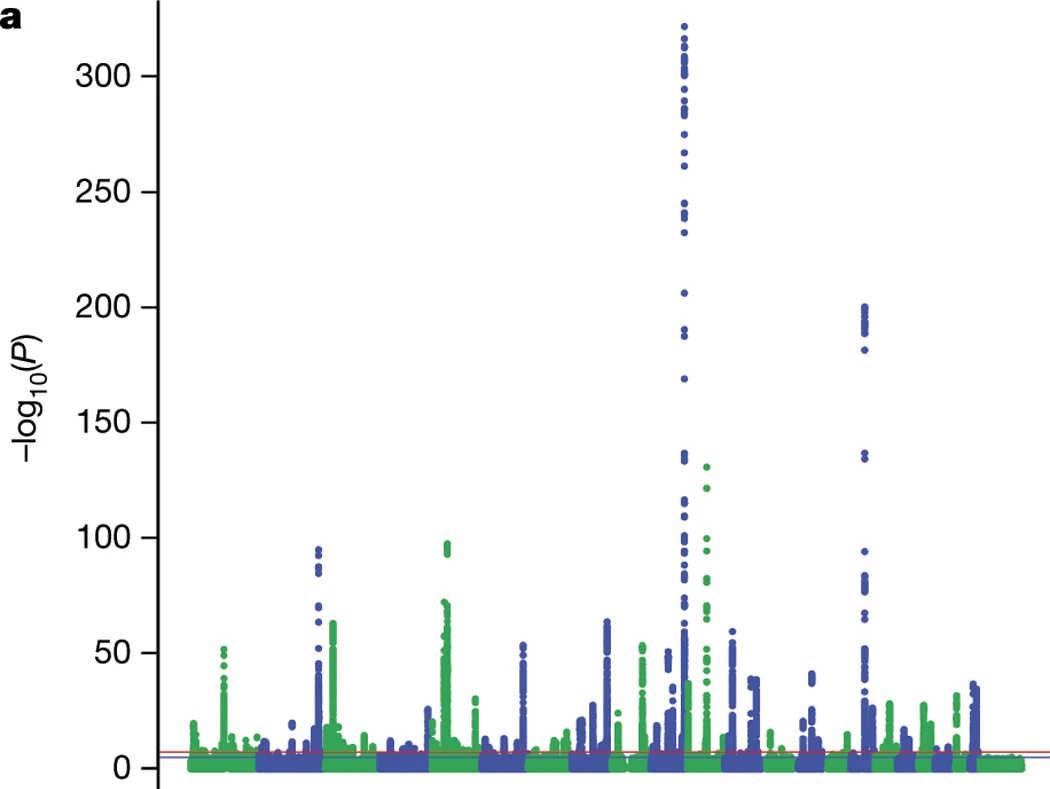
\includegraphics[width=0.25\textwidth]{{presentation_goldwp2022_paris/fig/41586_2017_Article_BFnature24284_Fig1_HTML}
\caption{GWAS for breast cancer}
\end{figure}

\begin{itemize}
\item Correlation between variants, ie. LD
\item Which cell types are causal to the disease?
\item Over 90\% GWAS variants fall in non-coding regions
\end{itemize}
%
\vfill
%
These points can be partially addressed by looking at eQTLs in different tissues

\let\thefootnote\relax\footnotetext{doi:10.3389/fgene.2020.00424}
\end{frame}


%%%%%%%%%%%%%%%%%%%%%%%%%%%%%%%%%%%%%%%%%%%%%%%%%%%%%%%%%%%%%%%%%%%%%%%%%%%%%%%%
\begin{frame}
\frametitle{Integration of GWAS and eQTL variants:  Colocalisation analysis}

\begin{figure}[!]
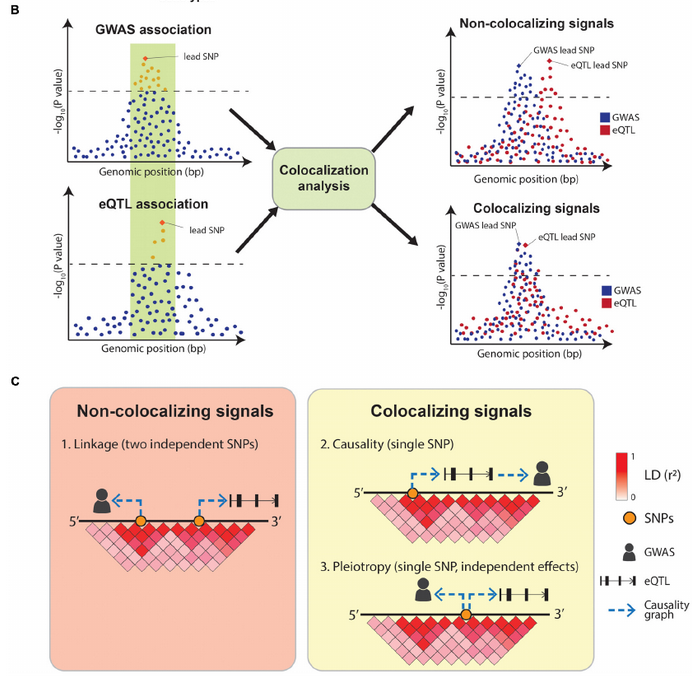
\includegraphics[width=0.6\textwidth]{presentation_goldwp2022_paris/fig/doi_10.3389_fgene.2020.00424_fig4.png}
\end{figure}

\let\thefootnote\relax\footnotetext{Cano-Gamez et al. 2020. doi:10.3389/fgene.2020.00424}
\end{frame}


\section{Objectives} %%%%%%%%%%%%%%%%%%%%%%%%%%%%%%%%%%%%%%%%%%%%%%%%%%%%%%%%%%%%%%

%%%%%%%%%%%%%%%%%%%%%%%%%%%%%%%%%%%%%%%%%%%%%%%%%%%%%%%%%%%%%%%%%%%%%%%%%%%%%%%%
\begin{frame}
\frametitle{Objectives}

\begin{itemize}
\item To identify eQTLs in immune cells that colocalise with frequent variants associated to cancer risk
\item To identify which immune cells are involved in cancer predisposition
\item To characterize these eQTLs involved in immune cells and cancer predisposition
\end{itemize}
\end{frame}

\section{Materials and Methods}

%%%%%%%%%%%%%%%%%%%%%%%%%%%%%%%%%%%%%%%%%%%%%%%%%%%%%%%%%%%%%%%%%%%%%%%%%%%%%%%%
\begin{frame}
\frametitle{Data and Algorithm}

\begin{itemize}
\item IEA OpenGWAS database
\item EBI eQTLs database
\item CRAN - Package coloc
\end{itemize}

\let\thefootnote\relax\footnotetext{https://gwas.mrcieu.ac.uk}
\end{frame}


\section{Conclusions, perspective and acknowledgements} %%%%%%%%%%%%%%%%%%%%%%%%%%%%%%%%%%%%%%%%%%%%%%%%%%%%%%%%%%%%%%

%%%%%%%%%%%%%%%%%%%%%%%%%%%%%%%%%%%%%%%%%%%%%%%%%%%%%%%%%%%%%%%%%%%%%%%%%%%%%%%%
\begin{frame}
\frametitle{Conclusions}

\begin{itemize}
\item A  colocalisation pipeline to link EBI Catalogue eQTLs and IEA OpenGWAS signals
\item Several colocalisation signals between immune cell eQTLs and cancer loci
\item Preliminary analyses of these colocalised signals
\end{itemize}

\end{frame}

%%%%%%%%%%%%%%%%%%%%%%%%%%%%%%%%%%%%%%%%%%%%%%%%%%%%%%%%%%%%%%%%%%%%%%%%%%%%%%%%
\begin{frame}
\frametitle{Perspectives}


\begin{itemize}
\item Use H1 as background dataset: H1=Causal SNP in cancer w/out eQTL
\item Statistics of cell type enrichments
\item Causal SNP characterization: Motif analyses
\item Other applications:
\begin{itemize}
\item Pleiotropy of eQTLs: eQTLs affecting two genes or same gene in two cell-types
\item Causality between other cell type eQTLs and diseases: Immunity and Covid-19
\end{itemize}
\end{itemize}

\end{frame}

%%%%%%%%%%%%%%%%%%%%%%%%%%%%%%%%%%%%%%%%%%%%%%%%%%%%%%%%%%%%%%%%%%%%%%%%%%%%%%%%
\begin{frame}
\frametitle{Acknowledgements}

\begin{itemize}
\item L\'eopoldine Lecerf (M1)
\item P Paul, P Rihet, M Michel
\item S Marquet, S Spicuglia
\item Funding:
\begin{itemize}
\item Institut Cancer et Immunologie (ICI)
\item Agence nationale de la recherche (ANR)
\end{itemize}
\end{itemize}

\end{frame}

\end{document}


